\documentclass[a4paper,11pt]{article}
\usepackage{amsmath,amsthm,amsfonts,amssymb,amscd,amstext,vmargin,graphics,graphicx,tabularx,multicol} \usepackage[french]{babel}
\usepackage[utf8]{inputenc}  
\usepackage[T1]{fontenc} 
\usepackage[T1]{fontenc}
\usepackage{amsmath,amssymb}
\usepackage{pstricks-add,tikz,tkz-tab,variations}
\usepackage[autolanguage,np]{numprint} 

\setmarginsrb{1.5cm}{0.5cm}{1cm}{0.5cm}{0cm}{0cm}{0cm}{0cm} %Gauche, haut, droite, haut
\newcounter{numexo}
\newcommand{\exo}[1]{\stepcounter{numexo}\noindent{\bf Exercice~\thenumexo} : \marginpar{\hfill /#1}}
\reversemarginpar


\newcounter{enumtabi}
\newcounter{enumtaba}
\newcommand{\q}{\stepcounter{enumtabi} \theenumtabi.  }
\newcommand{\qa}{\stepcounter{enumtaba} (\alph{enumtaba}) }
\newcommand{\initq}{\setcounter{enumtabi}{0}}
\newcommand{\initqa}{\setcounter{enumtaba}{0}}

\newcommand{\be}{\begin{enumerate}}
\newcommand{\ee}{\end{enumerate}}
\newcommand{\bi}{\begin{itemize}}
\newcommand{\ei}{\end{itemize}}
\newcommand{\bp}{\begin{pspicture*}}
\newcommand{\ep}{\end{pspicture*}}
\newcommand{\bt}{\begin{tabular}}
\newcommand{\et}{\end{tabular}}
\renewcommand{\tabularxcolumn}[1]{>{\centering}m{#1}} %(colonne m{} centrée, au lieu de p par défault) 
\newcommand{\tnl}{\tabularnewline}

\newcommand{\trait}{\noindent \rule{\linewidth}{0.2mm}}
\newcommand{\hs}[1]{\hspace{#1}}
\newcommand{\vs}[1]{\vspace{#1}}

\newcommand{\N}{\mathbb{N}}
\newcommand{\Z}{\mathbb{Z}}
\newcommand{\R}{\mathbb{R}}
\newcommand{\C}{\mathbb{C}}
\newcommand{\Dcal}{\mathcal{D}}
\newcommand{\Ccal}{\mathcal{C}}
\newcommand{\mc}{\mathcal}

\newcommand{\vect}[1]{\overrightarrow{#1}}
\newcommand{\ds}{\displaystyle}
\newcommand{\eq}{\quad \Leftrightarrow \quad}
\newcommand{\vecti}{\vec{\imath}}
\newcommand{\vectj}{\vec{\jmath}}
\newcommand{\Oij}{(O;\vec{\imath}, \vec{\jmath})}
\newcommand{\OIJ}{(O;I,J)}

\newcommand{\bmul}[1]{\begin{multicols}{#1}}
\newcommand{\emul}{\end{multicols}}


\newcommand{\reponse}[1][1]{%
\multido{}{#1}{\makebox[\linewidth]{\rule[0pt]{0pt}{20pt}\dotfill}
}}

\newcommand{\titre}[5] 
% #1: titre #2: haut gauche #3: bas gauche #4: haut droite #5: bas droite
{
\noindent #2 \hfill #4 \\
#3 \hfill #5

\vspace{-1.6cm}

\begin{center}\rule{6cm}{0.5mm}\end{center}
\vspace{0.2cm}
\begin{center}{\large{\textbf{#1}}}\end{center}
\begin{center}\rule{6cm}{0.5mm}\end{center}
}



\begin{document}
\pagestyle{empty}
\titre{Interrogation : Les probabilités}{Nom :}{Prénom :}{Classe}{Date}

\vspace*{0.5cm}


\exo{1} Donner la définition d'une expérience aléatoire.\\
\noindent \reponse[2]\\

\vspace*{0.5cm}

\exo{2} On fait tourner la roue de loterie ci-contre. Cette roue est équilibrée et est formée de huit secteurs identiques portant chacun une lettre.

\begin{center}

\includegraphics[scale=0.7]{interroroue.eps} 
\end{center}

\initqa \qa Quelles sont les issues de cette expérience aléatoire?\\
\noindent \reponse[2]\\

\qa Compléter les phrases suivantes :\\

- "Il y a . . . . chances sur  . . . . d'obtenir la lettre S"\\

- "Il y a . . . . chances sur  . . . . d'obtenir la lettre T"\\

\vspace*{0.5cm}

\exo{2} On lance un dé dodécaédrique (dé à douze faces) numéroté de 1 à 12.\\
Pour chacun des évènements ci-dessous, citer, lorsque
cela est possible, toutes les issues permettant de le réaliser.\\

\noindent \initqa \qa A : "Obtenir un nombre inférieur à 6".\\
\qa B : "Obtenir un multiple 5".\\
\qa C : "Obtenir un multiple de 2, de 3 et de 4".\\
\qa D : "Obtenir un nombre impair".\\

\noindent \reponse[6]

\newpage

\exo{2} Yann fait tourner la roue de la fortune. Cette roue est équilibrée.\\
 Lorsque que l'on tombe sur "Banqueroute" on ne gagne rien et on perd toute la somme que l'on a gagné auparavant.
 \bmul{2}

\begin{center}
\includegraphics[scale=0.6]{interroroue2.eps} 
\end{center}

\columnbreak

\initqa \qa Quelle est la probabilité de gagner 200 euros si on lance la roue?\\
\noindent \reponse[6]



\emul

\qa Quelle est la probabilité de ne rien gagner si on lance la roue?\\
\noindent \reponse[4]\\

\exo{3} 

Pour gagner à ce jeu, il faut tomber sur la couleur rouge. On a le choix entre une roulette, un dé et une urne contenant dix boules.\\

\includegraphics[scale=0.7]{exoproba1.eps}\\ 
Que faut-il choisir pour avoir le plus de chance de gagner : la roulette, le dé ou l'urne ? (\textbf{Justifier votre réponse avec des probabilités.})\\
 \reponse[8]





\end{document}
